\documentclass[tikz,border=8pt]{standalone}
\usepackage{amsmath}
\usepackage{pgfplots}
\pgfplotsset{compat=1.18}

\begin{document}
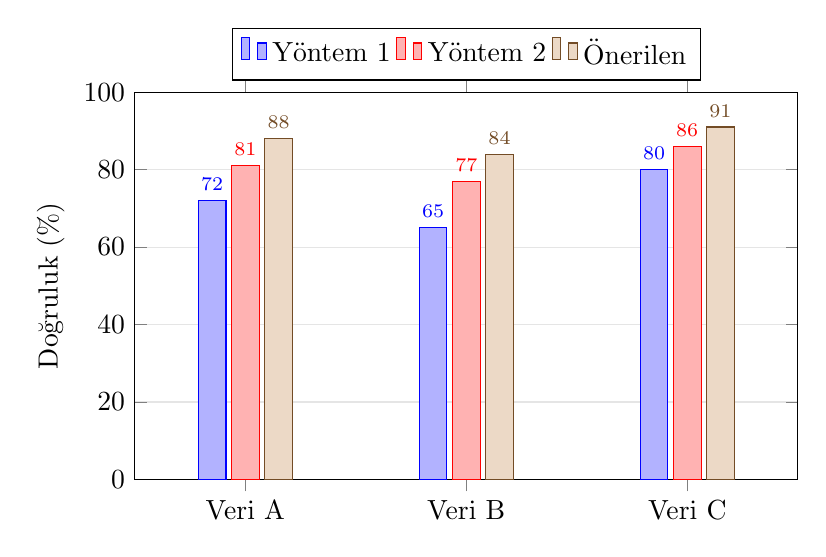
\begin{tikzpicture}
  \begin{axis}[
    ybar, bar width=10pt,
    width=10cm, height=6.5cm,
    ymin=0, ymax=100,
    ylabel={Doğruluk (\%)},
    symbolic x coords={Veri A, Veri B, Veri C},
    xtick=data,
    nodes near coords, nodes near coords style={font=\scriptsize},
    enlarge x limits=0.25,
    legend style={at={(0.5,1.03)}, anchor=south, legend columns=-1},
    grid=major, grid style={gray!20}, ymajorgrids=true, xmajorgrids=false,
  ]
    \addplot coordinates {(Veri A,72) (Veri B,65) (Veri C,80)};
    \addplot coordinates {(Veri A,81) (Veri B,77) (Veri C,86)};
    \addplot coordinates {(Veri A,88) (Veri B,84) (Veri C,91)};
    \legend{Yöntem 1, Yöntem 2, Önerilen}
  \end{axis}
\end{tikzpicture}
\end{document}
